\documentclass[11pt,a4paper]{article}
\usepackage{hyperref}
\usepackage[margin=2.5cm]{geometry}
\usepackage{amsmath, amsthm}
\usepackage{txfonts}
\usepackage{todonotes}
\usepackage{enumitem}
\usepackage{listings}
\usepackage[nameinlink]{cleveref}
\usepackage{microtype}
\usepackage{algorithm}
\usepackage{algpseudocode}
\usepackage{tikz}
\usepackage{mathtools}
\usepackage{catchfilebetweentags}
\usepackage{minted}
\usepackage{xcolor}

\definecolor{LightGray}{gray}{0.9}

\usemintedstyle{perldoc}
\newminted[code]{haskell}{bgcolor=LightGray}
\newminted[spec]{haskell}{}

\hypersetup{
  pdftitle={Storing the Cardano ledger state on disk},
  pdfborder={0 0 0},
  breaklinks=true
}

\newcommand{\htt}[1]{\mintinline[breaklines]{haskell}{#1}}

\usetikzlibrary{arrows.meta}
\usetikzlibrary{intersections}

\makeatletter
\tikzset{
    database/.style={
        path picture={
            \draw (0, 1.5*\database@segmentheight) circle [x radius=\database@radius,y radius=\database@aspectratio*\database@radius];
            \draw (-\database@radius, 0.5*\database@segmentheight) arc [start angle=180,end angle=360,x radius=\database@radius, y radius=\database@aspectratio*\database@radius];
            \draw (-\database@radius,-0.5*\database@segmentheight) arc [start angle=180,end angle=360,x radius=\database@radius, y radius=\database@aspectratio*\database@radius];
            \draw (-\database@radius,1.5*\database@segmentheight) -- ++(0,-3*\database@segmentheight) arc [start angle=180,end angle=360,x radius=\database@radius, y radius=\database@aspectratio*\database@radius] -- ++(0,3*\database@segmentheight);
        },
        minimum width=2*\database@radius + \pgflinewidth,
        minimum height=3*\database@segmentheight + 2*\database@aspectratio*\database@radius + \pgflinewidth,
    },
    database segment height/.store in=\database@segmentheight,
    database radius/.store in=\database@radius,
    database aspect ratio/.store in=\database@aspectratio,
    database segment height=0.1cm,
    database radius=0.25cm,
    database aspect ratio=0.35,
}
\makeatother

\theoremstyle{definition}
\newtheorem{property}{Property}
\newtheorem{definition}{Definition}
\newtheorem{lemma}{Lemma}
\newtheorem{assumption}{Assumption}
\newtheorem{corollary}{Corollary}
\newtheorem{proposal}{Proposal}
\newtheorem*{notation}{Notation}
\newtheorem{observation}{Key observation}
\newtheorem{failedattempt}{Failed attempt}

\newenvironment{bug}
  {\begin{quote} \textbf{Known bug}.}
  {\end{quote}}

\title{Storing the Cardano ledger state on disk\\
       {\large \sc UTxO-HD}}
\author{The Consensus Team}

\let\getss\gets
\renewcommand*{\gets}{\coloneqq}

\newcommand{\duncan}{\todo{Duncan suitable section.}}

\begin{document}

\maketitle

\tableofcontents

\section{Introduction}

The current and first version of UTxO-HD focuses only on moving the UTxO set to
the disk storage. This impacts the Consensus codebase almost in its entirety.
The Ledger and Node layers remain ignorant to this change on their side of the
interface and therefore the consensus side of the interfaces to the Ledger and
Node layers have to be slightly modified.

The reader is assumed to be familiar with the Consensus report \cite{report} and the general
architecture of the Consensus and Ledger layers.

Note that colorized \htt{Types} and \htt{functions} should appear in the
codebase so if in doubt, their Haddock documentation might provide more
information than this document.

\section{The LedgerDB}

\subsection{The basic definitions}

A \textbf{Ledger state at block $B$} is the state of the system after applying
all the blocks since Genesis up to block $B$ (included) on top of the Genesis
state. It contains the full state of the system, namely the UTxO set, the stake
delegations, chain state (nonces), etc. A full description of the Ledger state
can be found in the Ledger
specifications\footnote{\href{https://github.com/input-output-hk/cardano-ledger}{https://github.com/input-output-hk/cardano-ledger}}.

As we will be talking about the architectural changes in the code, we will be
referring to values of type \htt{LedgerState blk} as \textbf{Ledger states}.

Previously, a \htt{LedgerState blk} was a complete representation of the
concept of \textbf{Ledger state} as defined above.

\begin{code}
type LedgerState = Type -> Type
data family LedgerState blk
\end{code}

After UTxO-HD this is no longer the case as the UTxO set has been projected out
of said data-type. The data has then been split between the \emph{in-memory}
part (what we now informally call \emph{the ledger state without tables} or
\emph{the ledger state in memory}) and the \emph{ledger tables} which are
on-disk.

\begin{figure}[h]
  \centering
  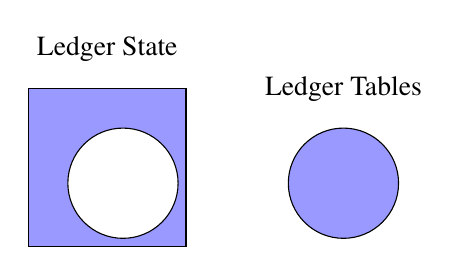
\begin{tikzpicture}
    \filldraw[fill=blue!40!white, draw=black] (0,0) rectangle (2,2);
    \filldraw[fill=white, draw=black] (1.2,0.8) circle (0.7);
    \node at (1,2.5) {Ledger State};
    \filldraw[fill=blue!40!white, draw=black] (4,0.8) circle (0.7);
    \node at (4,2) {Ledger Tables};
  \end{tikzpicture}
  \caption{The separation between the ledger state and the tables}
\end{figure}

The new types and kinds are these:

\begin{code}
type MapKind         = {- key -} Type -> {- value -} Type -> Type
type LedgerStateKind = MapKind -> Type

data family LedgerState blk :: LedgerStateKind

data family LedgerTables l :: LedgerStateKind
\end{code}

Ledger tables represent different views of the data that was moved to disk, in
particular with the first version of UTxO-HD only the UTxO set. A ledger state
has ledger tables attached to it which share the particular choice of \htt{MapKind} of the ledger state (different \htt{MapKind}s provide different
views). The ledger tables of a ledger state can be accessed via \htt{projectLedgerTables} and new tables can be attached to a ledger state via \htt{withLedgerTables}.

\begin{code}
projectLedgerTables :: IsMapKind mk => l mk  -> LedgerTables l mk
withLedgerTables    :: IsMapKind mk => l any -> LedgerTables l mk -> l mk
\end{code}

This is then concretized by the \htt{ApplyMapKind'} GADT which represents each
of the different views that ledger tables (and by extension ledger states) can
have on the UTxO set:

\begin{minted}{haskell}
data ApplyMapKind' :: MapKind' -> Type -> Type -> Type where
  ApplyDiffMK     :: !(Diff    k v)                -> ApplyMapKind' DiffMK'     k v
  ApplyEmptyMK    ::                                  ApplyMapKind' EmptyMK'    k v
  ApplyKeysMK     :: !(Keys    k v)                -> ApplyMapKind' KeysMK'     k v
  ApplySeqDiffMK  :: !(DiffSeq k v)                -> ApplyMapKind' SeqDiffMK'  k v
  ApplyTrackingMK :: !(Values  k v) -> !(Diff k v) -> ApplyMapKind' TrackingMK' k v
  ApplyValuesMK   :: !(Values  k v)                -> ApplyMapKind' ValuesMK'   k v
\end{minted}

The intuition about what these constructors represent can be easily described:

\begin{itemize}
  \item A value of type \htt{LedgerState blk EmptyMK} can project tables of
        type \htt{LedgerTables (LedgerState blk) EmptyMK} which holds an
        empty constructor \htt{ApplyEmptyMK}
  \item A value of type \htt{LedgerState blk KeysMK} can project tables of
        type \htt{LedgerTables (LedgerState blk) KeysMK} which holds a set of
        keys. For the UTxO set case in particular, a set of \htt{TxIn}s.
  \item A value of type \htt{LedgerState blk DiffMK} can project tables of
        type \htt{LedgerTables (LedgerState blk) DiffMK} which holds a map
        from keys to diff entries. Diff entries are computed by comparing two
        \htt{ValuesMK} tables to find out which keys have been
        removed/inserted/updated from one map to another. For the UTxO set case
        in particular, as entries cannot be updated nor they can be inserted
        twice, this holds a map from \htt{TxIn}s to whether that key was
        inserted (and with what value) or whether it was deleted.
  \item A value of type \htt{LedgerState blk ValuesMK} can project tables of
        type \htt{LedgerTables (LedgerState blk) ValuesMK} which holds a map
        from keys to values. For the UTxO set case in particular, a map of
        \htt{TxIn}s to \htt{TxOut}s.
  \item A value of type \htt{LedgerState blk TrackingMK} can project tables
        of type \htt{LedgerTables (LedgerState blk) TrackingMK} which is a
        sum of a \htt{ValuesMK} table and a \htt{DiffMK} table.
  \item A value of type \htt{LedgerState blk SeqDiffMK} can project tables of
        type \htt{LedgerTables (LedgerState blk) SeqDiffMK} which hold a
        sequence of differences sorted by the slot number of the block that
        produced them, contained in a fingertree. The exact implementation of
        this container is a concern of the {\tt
        anti-diff}\footnote{\href{https://github.com/input-output-hk/ouroboros-network/tree/feature/utxo-hd/anti-diff}{https://github.com/input-output-hk/ouroboros-network/tree/feature/utxo-hd/anti-diff}}
        package.
\end{itemize}

The following ghci pseudo-examples show representations of each type of tables:

\begin{code}
  > let l  = foo :: LedgerState blk EmptyMK
  > let k  = l `withLedgerTables` ApplyKeysMK (fromList [10, 12])
  > let v1 = l `withLedgerTables` ApplyValuesMK (fromList [(0, 0), (1, 1)])
  > let v2 = l `withLedgerTables` ApplyValuesMK (fromList [(1, 1), (2, 4)])
  > printTables l
  Empty
  > printTables k
  ApplyKeysMK   (fromList [10, 12])
  > printTables v1
  ApplyValuesMK (fromList [(0,0), (1,1)])
  > printTables (v2 `diff` v1)
  ApplyDiffMK   (fromList [(0, Delete), (2, Insert 4)])
  > v1 `applyDiffs` (v2 `diff` v1) == v2
  True
\end{code}

\subsection{A ledger state with no tables still has values}
\begin{observation}
  \emph{The ledger states defined above use \textbf{the same in-memory part}
    (namely the in-memory part of \texttt{l}).} \emph{The part of the Ledger
    state which is not the Ledger tables is unaffected by the particular choice
    of \texttt{ApplyMapKind}.}
\end{observation}

This is a crucial observation: \texttt{l} is \textbf{not} dependent on the
tables. As mentioned in the beginning of this section, the Ledger interface side
of the Consensus-Ledger interface didn't change so we have to end up providing
data in a structure equivalent to the one before UTxO-HD. In particular, there
must be a field on the data structure hierarchy that builds a
\htt{LedgerState blk mk} that must contain the UTxO set and nothing prevents
us from having some data there. In particular, the following ledger state is well-shaped:

\begin{code}
  > let (txin, txout) = ... :: (TxIn blk, TxOut blk)
  > let l' = SomeLedgerStateConstructor {
      .. = {
          ..
        , utxoSet = Map.singleton (txin, txout)
        }
      } `withLedgerTables` ApplyEmptyMK :: LedgerState blk EmptyMK
\end{code}

(Just for simplicity we are assuming \htt{TxIn} and \htt{TxOut} depend on
the block type although this is not the case in reality). One can think that
this value makes no sense as it holds a UTxO set despite the tables being empty.

The fact that it is allowed to have values inside the ledger state even if the
tables are declared as empty is only intended to manifest when we are about to or
have just interfaced with the ledger. Once the value goes into the Consensus
layer it is expected that the in-memory part of the ledger state holds no
values.

The reason behind this fact is that the Ledger layer types are wrapped by
Consensus types representing the Ledger state, and despite the tables being part
of the latter, they are not part of the former. As an example, one can see the
\htt{LedgerState (ShelleyBlock proto era)} definition before UTxO-HD:

\begin{code}
  data instance LedgerState (ShelleyBlock proto era) = ShelleyLedgerState {
      shelleyLedgerTip        :: !(WithOrigin (ShelleyTip proto era))
    , shelleyLedgerState      :: !(SL.NewEpochState era)
    , shelleyLedgerTransition :: !ShelleyTransition
  }
\end{code}

The Ledger layer defines \htt{SL.NewEpochState} (as defined in the Ledger formal
specifications) and the Consensus layer wraps this type in its own
\htt{LedgerState} data-type instance. Now, after UTxO-HD, this datatype has
evolved into the following:

\begin{code}
data instance LedgerState (ShelleyBlock proto era) mk = ShelleyLedgerState {
      shelleyLedgerTip        :: !(WithOrigin (ShelleyTip proto era))
    , shelleyLedgerState      :: !(SL.NewEpochState era)
    , shelleyLedgerTransition :: !ShelleyTransition
    , shelleyLedgerTables     :: !(LedgerTables (LedgerState (ShelleyBlock proto era)) mk)
    }
\end{code}

The Ledger layer still operates with the same types as before UTxO-HD so we are
forced to relocate whatever data we want to pass to the Ledger in the
appropriate fields, and also extract the data out again. This is achieved by the
functions declared in the \htt{StowableLedgerTables} class.

\begin{code}
class StowableLedgerTables (l :: LedgerStateKind) where
  stowLedgerTables     :: l ValuesMK -> l EmptyMK
  unstowLedgerTables   :: l EmptyMK  -> l ValuesMK
\end{code}

So now, using the same values as in previous code snippets:
\begin{code}
  > printUtxosInNewEpochState l'
  fromList [(txin, txout)]
  > printTables l'
  Empty
  > printTables (unstowLedgerTables l')
  ApplyValuesMK (fromList [(txin, txout)])
  > printUtxosInNewEpochState (unstowLedgerTables l')
  fromList []
  > stowLedgerTables (unstowLedgerTables l') == l'
  True
\end{code}

Note that the hole left by extracting the tables is not really a hole as
pictured earlier in this section, but instead it is filled with an empty
\texttt{Data.Map} container.

\subsection{Notation}

\begin{itemize}
  \item We will denote a value of type \htt{LedgerState blk mk} as a tuple
        $(L, T)$ where $L$ represents the Ledger layer part of the ledger state
        (i.e. the \htt{SL.NewEpochState}) and $T$ represents the tables. As
        seen above, a value of type \htt{LedgerState blk mk} has some other
        data inside, for example the Header state. As this is not relevant for
        UTxO-HD we will omit that extra data.

  \item We will use the superscript $L^{s}$ when we mean that the ledger state
        $L$ has been ticked to the slot $s$.

  \item Whenever we want to specify the actual values that have been
        \texttt{stowed} into a Ledger layer value, we will use a subscript with
        the tables that were injected, i.e.
        \htt{stowLedgerTables}$(L, V) \hookrightarrow (L_{V}, \emptyset)$, where
        $\emptyset$ represents the empty ledger tables, or simply $L_{v}$.

  \item Applying differences to values will be denoted by the left triangle
        $\triangleleft : $ \htt{ValuesMK} $\times$ \htt{DiffMK} $\rightarrow$ \htt{ValuesMK}.

  \item Identifiers that appear \htt{colorized} in the pseudocode algorithms are
        actual names of functions/fields used in the real codebase so they
        should be searchable.
\end{itemize}

\subsection{In memory design}

The ledger database was traditionally made of \texttt{AnchoredSeq}s of ledger
states, but as of UTxO-HD this is no longer the case. We hold instead what we
call \htt{DbChangelog} which is an \htt{AnchoredSeq} of \emph{in-memory}
ledger states and the corresponding sequence of differences to the tables:

\begin{code}
data DbChangelog l = DbChangelog {
    changelogDiffAnchor      :: !(WithOrigin SlotNo)
  , changelogDiffs           :: !(LedgerTables l SeqDiffMK)
  , changelogImmutableStates ::
      !(AnchoredSeq
          (WithOrigin SlotNo)
          (l EmptyMK)
          (l EmptyMK)
       )
  , changelogVolatileStates  ::
      !(AnchoredSeq
          (WithOrigin SlotNo)
          (l EmptyMK)
          (l EmptyMK)
       )
  }
\end{code}

The sequence of differences held in the \htt{DbChangelog} correspond to the
differences produced when going from one of the states in the fragments to the
next one, i.e. the first entry of differences belongs to the differences produced
when applying the first block which produced the first element in the sequence
of states, and so on.

There is one important observation here: the sequence of differences is relative
to some initial (or anchor) set of values. This set of values lives in the disk
and is what will be refered as the \textbf{Backing store} from now on. It
represents the UTxO values at the ledger state referenced as the anchor of the
sequence of immutable states.

\begin{figure}[h]
  \centering
  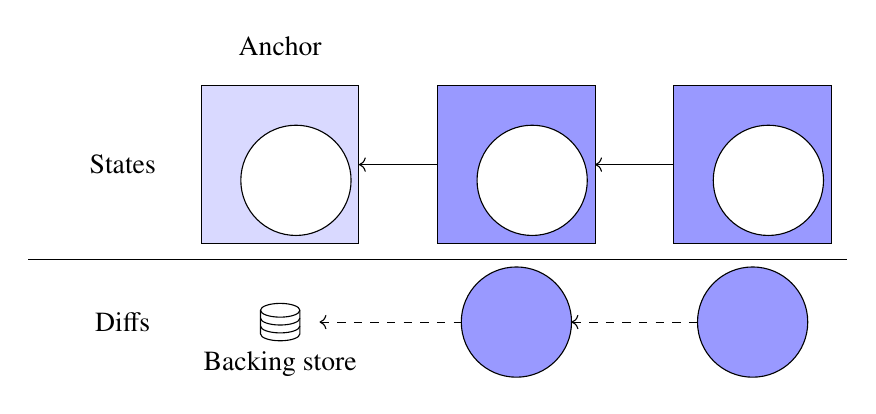
\begin{tikzpicture}
    \node at (-1,1) {States};
    \node at (1,2.5) {Anchor};
    \draw (-2.2,-0.2) -- (8.2,-0.2);
    \filldraw[fill=blue!15!white, draw=black] (0,0) rectangle (2,2);
    \filldraw[fill=white, draw=black] (1.2,0.8) circle (0.7);
    \draw[<-] (2,1) -- (3,1);
    \filldraw[fill=blue!40!white, draw=black] (3,0) rectangle (5,2);
    \filldraw[fill=white, draw=black] (4.2,0.8) circle (0.7);
    \draw[<-] (5,1) -- (7,1);
    \filldraw[fill=blue!40!white, draw=black] (6,0) rectangle (8,2);
    \filldraw[fill=white, draw=black] (7.2,0.8) circle (0.7);

    \filldraw[fill=blue!40!white, draw=black] (4,-1) circle (0.7);
    \filldraw[fill=blue!40!white, draw=black] (7,-1) circle (0.7);
    \node at (-1,-1) {Diffs};
    \node[database,label=below:Backing store] at (1, -1){};
    \draw[<-,dashed] (1.5,-1) -- (3.3,-1);
    \draw[<-,dashed] (4.7,-1) -- (6.3, -1);
  \end{tikzpicture}
  \caption{The DbChangelog}\label{fig:dbch}
\end{figure}

In order for the ledger database to not grow indefinitely, we need to prune it
from time to time. We define the security parameter $k$ ($= 2160$ on mainnet) as
the number of ledger states that we will consider volatile. This means that the
states which are more than $k$ distance from the tip of our current selection
will be considered \textbf{immutable} and we can garbage collect them, pruning
the database.

Before UTxO-HD, pruning the ledger database was done just by dropping items from
the beginning of the sequence of immutable states. However, now we need to also
flush their corresponding differences into the Backing store in order to keep
it in sync with the DbChangelog.

Now that we have seen how the differences are carried around, there is one important observation to make:

\begin{observation}
  \label{ko1}
  \emph{The way to mimick a pre-UTxO-HD full ledger state (in which we would be
    able to query for every utxo in existence) is by holding the initial set of
    values (Backing store) and a sequence of differences up to this ledger
    state}.
\end{observation}

So what previously was a standalone value (before UTxO-HD, every ledger state
contained all utxos in existence at that point in time) has now evolved into a
compound value that requires coordination between the backing store and the
\htt{DbChangelog}.

Because of the above, we cannot flush the \htt{DbChangelog} into the Backing
store at will, as we could fall into inconsistent states. As described in
\textbf{Key observation \ref{ko1}}, in order to preserve the consistency needed
to mimick a complete ledger state there will be moments in which we cannot let
the Ledger database perform side effects on the backing store. In particular the
following observation is important:

\begin{observation}
  \label{ko2}
  \emph{Whenever we acquire a LedgerState on top of which we plan to apply
    transactions (or blocks) for which we still don't have retrieved the tables
    of needed values, we need to also acquire the corresponding \htt{DbChangelog} and
    hold the flush lock in read mode in order to have a consistent view of the
    UTxO set}.
\end{observation}

\subsection{Backing store definition and implementations}

The \textbf{backing store} is some stateful storage which holds the UTxO values
as of some block in the immutable database. It is unique, i.e. there is only one
in the system. It has to support the following interface:

\begin{code}
data BackingStore m keys values diff = BackingStore {
    -- | Close the backing store
    --
    -- Other methods throw exceptions if called on a closed store.
    bsClose       :: !(m ())
    -- | Create a persistent copy
    --
    -- Each backing store implementation will offer a way to initialize itself
    -- from such a path.
    --
    -- The destination path must not already exist. After this operation, it
    -- will be a directory.
  , bsCopy        :: !(FS.SomeHasFS m -> BackingStorePath -> m ())
    -- | Open a 'BackingStoreValueHandle' capturing the current value of the
    -- entire database
  , bsValueHandle :: !(m ( WithOrigin SlotNo
                         , BackingStoreValueHandle m keys values))
    -- | Apply a valid diff to the contents of the backing store
  , bsWrite       :: !(SlotNo -> diff -> m ())
}

-- | An ephemeral handle to an immutable value of the entire database
--
-- The performance cost is usually minimal unless this handle is held open too
-- long.
data BackingStoreValueHandle m keys values = BackingStoreValueHandle {
    -- | Close the handle
    --
    -- Other methods throw exceptions if called on a closed handle.
    bsvhClose     :: !(m ())
    -- | See 'RangeQuery'
  , bsvhRangeRead :: !(RangeQuery keys -> m values)
    -- | Read the given keys from the handle
    --
    -- Absent keys will merely not be present in the result instead of causing a
    -- failure or an exception.
  , bsvhRead      :: !(keys -> m values)
  }
\end{code}

As mentioned above, the Backing store corresponds to the UTxO set at some {\bf
  immutable} state. It follows then that as it is immutable, no rollback will
ever be performed: we will only flush newer differences which become immutable,
i.e. we will only \emph{move forward} on the chain of blocks. To identify which
ledger state the backing store is in sync with, we provide a \htt{SlotNo} that
will be always increasing.

The interface above is in particular, concretized by the \htt{LedgerBackingStore} newtype:

\begin{code}
newtype LedgerBackingStore m l = LedgerBackingStore
    (BackingStore.BackingStore m
      (LedgerTables l KeysMK)
      (LedgerTables l ValuesMK)
      (LedgerTables l DiffMK)
    )
\end{code}

We provide three different implementations of a Backing store:

\begin{description}
  \item[InMemory] a super straightforward implementation which is
        essentially a \htt{TVar} holding both a \htt{WithOrigin SlotNo}
        and a \htt{LedgerTables l ValuesMK}.

  \item[LMDB\footnote{\href{http://www.lmdb.tech/doc/}{http://www.lmdb.tech/doc/}}] which uses the
        key-value database to store tables of values (\htt{LedgerTables
        l ValuesMK}) serialized. The \htt{SlotNo} is stored in a
        separate unitary table.

  \item[LSM Trees] TBD

\end{description}

\section{Interface with the Ledger}

The Ledger layer has not been modified for UTxO-HD and therefore the ledger
states that we provide to the ledger must be indistinguishable from those before
UTxO-HD in what matters to the Ledger rules that will be executed. In order to
understand why some actions are allowed, one has to interiorize the following
\textbf{Key observations}:

\begin{observation}
  \emph{In order to succesfully apply a block, the UTxO set inside the ledger state
  only needs to contain the entries consumed by the transactions in the block.This is also true when speaking about transaction application: only the inputs
  consumed by the transaction are actually needed by the Ledger.}
\end{observation}

\begin{observation}
  \emph{In order to succesfully tick a ledger state not through an era
    transition, the UTxO set can be empty as the ledger rules don't look at it.}
\end{observation}

\begin{observation}
  \emph{Ticking a ledger state through an era transition might require some
    entries on the UTxO set and can produce changes in them, therefore ticking
    has to be considered as producing tables with differences. Examples will be
    seen in Section~\ref{sec:eratrans}. }
\end{observation}

The reasoning behind these observations can be seen in the Cardano ledger formal specifications\footnote{\href{https://github.com/input-output-hk/cardano-ledger}{https://github.com/input-output-hk/cardano-ledger}}, by inspecting the rules mentioned.

The sequence of actions for ticking and applying a block $B$ at slot $s$ on top
of a ledger databse whose tip is the state $L$ is then easily described by
\textbf{Algorithm \ref{alg:tickandapply}}.

\begin{algorithm}[h]
  \caption{Tick and apply}
  \label{alg:tickandapply}
  \begin{algorithmic}[1]
    \Procedure{\htt{applyBlock}}{$DB ::$ \htt{LedgerDB}$, B ::$ \htt{Block}}
    \State $(L, \emptyset) \gets$ \htt{ledgerDbCurrent}$(DB)$
    \State $(L^{s}, V_{\tt TICK}) \gets$ \htt{unstowLedgerTables}$(\texttt{TICK}(L, s))$
    \State $D_{s} \gets$ \htt{diff}$(V_{\tt TICK}, \emptyset)$ \Comment{Empty unless ticking on an era transition}
    \Statex
    \State $V_{in} \getss$ \htt{bsRead}$($\htt{getBlockKeySets}$(B)) \triangleleft \left.{\tt DbChangelog}\right|_{\dots\texttt{Pred}(B)} \triangleleft D_{s}$
    \Statex \Comment{$\texttt{Pred}(B)$ stands for \emph{$B$'s predecesor}}
    \State $L^{s}_{V_{in}} \gets$ \htt{stowLedgerTables}$(L^{s},V_{in})$
    \State $(L', V_{out}) \gets$ \htt{unstowLedgerTables}$(\texttt{APPLY}(B, L^{s}_{V_{in}}))$
    \State $D_{B} \gets$ \htt{diff}$(V_{out}, V_{in})$
    \Statex{}
    \State \Return $(L', D_{s} \diamond D_{B})$
    \EndProcedure
 \end{algorithmic}
\end{algorithm}

\section{Anti-diffs}

\subsection{The FingerTree problem}

\subsection{Algebra of differences}

\subsection{It is a semigroupoid!}

\section{The Mempool}

\subsection{Definition and design}

The mempool is the set of transactions that should be included in the next
block. In principle this is a \emph{set} of all the transactions that we receive
from our peers. We can consider the mempool as an ubiquitous container of
transactions that is accessed from multiple places at the same time and should
be able to provide a list of transactions (what we call a \emph{snapshot}) which
are valid on top a of a given state, possibly (and usually) on top of the current LedgerDB's
tip.

As transactions arrive, the mempool will try to validate them on the current
ledger state (the current LedgerDB's tip) so that if the mempool is asked for a
snapshot on top of that ledger state (which is the case most of the times), it
already has a cached version ready to be provided. If instead it is asked for a
snapshot on top of a different ledger state, it will have to revalidate all the
\emph{previously valid} transactions on top of said ledger state.

The interface to the mempool is roughly as follows:

\begin{code}
data Mempool m blk idx = Mempool {
   tryAddTxs      :: WhetherToIntervene
                  -> [GenTx blk]
                  -> m ( [MempoolAddTxResult blk]
                       , [GenTx blk]
                       )
 , syncWithLedger :: m (MempoolSnapshot blk idx)
 , getSnapshotFor :: SlotNo
                  -> TickedLedgerState blk DiffMK
                  -> MempoolChangelog blk
                  -> m (MempoolSnapshot blk idx)
 , ...
}
\end{code}

The \htt{MempoolChangelog} datatype is the result of dropping the sequences of \htt{l EmptyMK} ledger states from a normal \htt{DbChangelog}.

At every point in time, the mempool is anchored on top of the current selection
of the ChainDB, and a background thread\footnote{See
  \href{https://github.com/input-output-hk/ouroboros-network/tree/feature/utxo-hd/ouroboros-consensus/src/Ouroboros/Consensus/Background.hs}{this file}}
is in charge of making sure that whenever the tip changes, the mempool gets
revalidated.

The mempool holds a \emph{virtual ledger state} resulting from ticking the
anchor ledger state to some tentative slot number and then applying all the
previously known-valid transactions on top of it. Now that UTxO-HD has redefined
what a ledger state is, the mempool holds a (Ledger's layer) virtual ledger
state and a view on the sequence of differences to the ledger tables coming from
the \htt{LedgerDB}'s \htt{DbChangelog} that would correspond to that ledger
state. This is shown by the data held in the Mempool's \htt{InternalState}:

\begin{code}
data InternalState blk = IS {
   -- | Transactions currently in the mempool
   isTxs          :: !(TxSeq (Validated (GenTx blk)))

   -- | The cached ledger state after ticking the ledger state identified by
   -- 'isTip' to 'isSlotNo' and applying the transactions in the Mempool
   -- against this ledger state. New transactions will be validated by
   -- applying them on top of 'isLedgerState'.
 , isLedgerState  :: !(TickedLedgerState blk DiffMK)

   -- | The changelog as captured on the last sync with the ledger.
 , isDbChangelog  :: !(MempoolChangelog blk)
   ...
}
\end{code}

(Note that the prefix $is$ stands for \emph{internal state} and not the verb \emph{to be})

This internal state is kept inside a \htt{StrictTMVar}\footnote{the different operations on the mempool have to make
sure that there is no path in which the \htt{TMVar} would remain empty (and
therefore produce a deadlock)} by the
\htt{MempoolEnv}.

It is important to note that this has to be a \htt{TVar} because concurrent
addition of transactions have to be done in atomic steps, and it has to be a
\htt{MVar} because we need to perform \htt{IO} while the contents must
remain non-updateable by other actors. In particular, most of the operations on
the mempool follow this pattern:

\begin{algorithm}
  \caption{Pattern of mempool operation}
  \begin{algorithmic}[1]
    \Procedure{MempoolOp}{$M :: $ \htt{Mempool}}
    \State $\texttt{is} \getss$ \htt{atomically}$($\htt{takeTMVar} $M)$
    \State $x \getss \texttt{someIO}(\texttt{is})$
    \State \htt{atomically}$(\texttt{doSomething}(x) >>=$ \htt{putTMVar} $M)$
    \EndProcedure
 \end{algorithmic}
\end{algorithm}

The \texttt{someIO} is usually reading UTxO values from the Backing store, and
then \texttt{doSomething} is the actual operation that we want to perform more
or less as it was done before UTxO-HD.

\subsection{Operations}

\subsubsection{Adding transactions}

The problem of applying transactions described in \textbf{Algorithm~\ref{alg:addtx}} is then solved in a very straightforward
way, quite similarly to applying a block.

\begin{algorithm}
  \caption{Adding transactions}
  \label{alg:addtx}
  \begin{algorithmic}[1]
    \Procedure{\htt{tryAddTxs}}{$DB ::$ \htt{LedgerDB}$, M ::$ \htt{MempoolEnv}$, txs@(tx:next) :: [$\htt{Tx}$]$}
    \State $is \getss$ \htt{readTVar}(\htt{mpStateVar} $M$)
    \State $(L^{s},D_{M}) \gets$ \htt{isLedgerState} $is$
    \State $V_{in} \getss$ \htt{bsRead}$_{DB}($\htt{getTransactionKeySets}$(tx)) \triangleleft \texttt{isDbChangelog}(is) \triangleleft D_{M}$
    \If {\texttt{error?}}
    \State \htt{implSyncWithLedger}$(DB,M)$ \Comment{this will update the internal state}
    \State \htt{tryAddTxs}$(DB,M,txs)$
    \Else
    \State $L^{s}_{V_{in}} \gets$ \htt{stowLedgerTables}$(L^{s},V_{in})$
    \State $(L^{s},V_{out}) \gets$ \htt{unstowLedgerTables}$(\texttt{APPLY}(tx, L^{s}_{V_{in}}))$
    \If {$\neg$ \texttt{error?}}

    \State $D_{tx} \gets$ \htt{diff}$(V_{out}, V_{in})$
    \State $is' \gets is[$\htt{isLedgerState} $ \mapsto (L^{s}, D_{M} \diamond D_{tx}), $ \htt{isTxs} $\mapsto tx:$ \htt{isTxs} $is]$
    \State \htt{writeTVar} $($\htt{mpStateVar} $M)~is'$
    \EndIf
    \State \htt{tryAddTxs}$(DB, M, next)$
    \EndIf
    \EndProcedure
 \end{algorithmic}
\end{algorithm}

The resulting ledger state is stored in the Mempool's internal state and the
transaction is added to the list of valid transactions. Of course, in the same
way as before UTxO-HD, when the transaction fails to apply, the result is
discarded.

This process mimicks the process before UTxO-HD in which the mempool held a
complete ledger state with the whole UTxO set in it and applied transactions to
it. Now only one more special case arises which was not needed prior to these
changes: the disk anchor moving.

If \htt{bsRead} fails to retrieve the values because the \htt{DbChangelog} held
by the mempool got out of sync with the one on the disk, we are forced to
perform a sync with the ledger in order to get an up to date \htt{DbChangelog}.
Note that we could in principle just retry until the mempool gets synced by the
background thread, but this could lead to starvation of threads. Calling
\htt{implSyncWithLedger} here ensures that the sync is performed and the next
call done by the background thread will be super cheap as the mempool would be
in sync already.

\subsubsection{Syncing with the ledger}

Just as mentioned, syncing with the ledger database is a super cheap operation
when the mempool is already in sync, so several calls to
\htt{implSyncWithLedger} should be idempotent if the ledger database didn't
change.

There are two elements that could have gone out of sync, or maybe even both of
them: the tip of the LedgerDB and the \htt{MempoolChangelog}.

In case the \htt{MempoolChangelog} in the mempool has gotten out of sync with
the \htt{DbChangelog} in the LedgerDB, as the anchor of the Backing store
belongs to the immutable part of the ledger database, it can only move forward,
either along the same chain that is being represented currently on the mempool,
or on a different fork.

Depending on whether or not the tip changed we might have to need to revalidate
the transactions in the mempool. Note that if the tip didn't change but the
changelog changed, it can only be the case that the anchor moved along the same
selection of blocks, and therefore the transactions are still valid.

If the tip did change, then we are forced to get a new \htt{MempoolChangelog}
and just revalidate all the transactions.

The complete algorithm for syncing with the ledger database can be seen in \textbf{Algorithm~\ref{alg:sync}}.

\begin{algorithm}
  \caption{Syncing with the ledger database}
  \label{alg:sync}
  \begin{algorithmic}[1]
    \Procedure{\htt{implSyncWithLedger}}{$DB :: \texttt{LedgerDB},M :: \texttt{Mempool}$}
    \State $\texttt{acquireRead}(DB)$
    \State $(L, \texttt{Diffs}) \gets$ \htt{getCurrentLedgerAndChangelog}$_{DB}$
    \If {$L = $ \htt{isLedgerState} $M$}
    \If {${\tt Diffs} =$ \htt{isDbChangelog} $M$}
        \State $\texttt{releaseRead(DB)}$
    \State \Return $M$ \Comment{Nothing to do}
    \Else
    \State $\texttt{releaseRead(DB)}$
    \State \Return $M[$ \htt{isDbChangelog} $\mapsto {\tt Diffs}]$ \Comment{Backing store moved forward}
    \EndIf
    \Else \Comment{Need to revalidate as tip changed}
    \State $M' \gets M [$ \htt{isLedgerState} $\mapsto L,$ \htt{isDbChangelog} $\mapsto \texttt{Diffs}] $
    \State $M'' \gets \texttt{fold}(\texttt{revalidateMempool}(DB), M', \texttt{isTxs}_{M})$
    \State $\texttt{releaseRead(DB)}$
    \State \Return $M''$
    \EndIf
    \EndProcedure
 \end{algorithmic}
\end{algorithm}

\subsubsection{Getting snapshots for forging}

When the node is forging blocks, in case it is the slot leader for the current
slot, it will ask the mempool for a list of valid transactions on top of its
current best block (usually the tip of the ChainDB). This \emph{might} imply
revalidating the transactions in case the mempool was not synced with this
ledger state.

As mentioned in \textbf{Key observation \ref{ko2}}, we are in a situation in
which we have a concrete ledger state on top of which we maybe need to apply
transactions for which we still don't have forwarded the values yet. This
implies that it is mandatory that we hold the read lock while performing this
operation to ensure that the Backing store doesn't move.

The forging logic\footnote{search for \htt{forkBlockForging}} will grab a
\htt{DbChangelog} as it starts and we need to make sure it remains valid at
least up to the point when we consult the mempool for a snapshot.

It is crucial to note that the write lock will be requested when performing a
flush of differences and it is the case that \htt{addBlock} (which is called by
\htt{addBlockSync} as the last step of the forging logic) might trigger this
situation, and therefore we cannot be holding the read lock when we reach that
point.

\begin{observation}
  \emph{The flushing lock (acquired at the beginning of the forging loop) must
    be released before trying to add the produced block to the ChainDB or
    otherwise we will face a deadlock.}
\end{observation}

On the mempool side, the logic for retrieving the snapshot is pretty basic,
consisting only on either returning the already known list of valid transactions
if we happen to already be in sync with the best ledger state, or revalidate the
transactions on top of the given ledger state considering the given diffs, in
a style similar to what was done in \textbf{Algorithm \ref{alg:sync}}.

\subsection{TxSubmission protocols}

No changes were needed on the TxSubmission protocols, so the documentation from
the Network team and the mini-protocol specifications are still fully
applicable.

\section{Cardano Blocks}

Apart from all mentioned above, the Cardano case has some design decisions that
somewhat bend the rules described.

\subsection{Byron tables}

The Byron ledger is considered somewhat \emph{obsolete} in the sense that no
more blocks will be produced by the Byron ledger ever, and therefore the easiest
approach for it was to just ignore the UTxO-HD concepts and have no ledger
tables at any moment. This gave rise to the following typeclass:

\begin{code}
class InMemory l where
  convertMapKind :: l mk -> l mk'
\end{code}
Which basically states that for this ledger, modifying the type of the ledger
tables is a noop. Among the Cardano ledgers, this is only true for Byron ( it is
also true for test blocks, but that is not the concern of this document).

So in particular, the type of the tables is a phantom type on Byron:

\begin{code}
data instance LedgerState ByronBlock mk = ByronLedgerState {
  ...
}
\end{code}

\subsection{Shelley tables}

Starting on Shelley and onwards (i.e. for all the ``Shelley eras'' which are the eras that use the \htt{NewEpochState}), the type of the ledger state is the same:

\begin{code}
data instance LedgerState (ShelleyBlock proto era) mk = ShelleyLedgerState {
  ...
  shelleyLedgerState      :: !(SL.NewEpochState era)
  ...
, shelleyLedgerTables     ::
      !(LedgerTables (LedgerState (ShelleyBlock proto era)) mk)
}
\end{code}

The tables are then defined as maps/sets parametrized by the actual \texttt{era}:

\begin{code}
newtype LedgerTables (LedgerState (ShelleyBlock proto era)) mk =
  ShelleyLedgerTables {
    shelleyUTxOTable :: mk (SL.TxIn (EraCrypto era)) (Core.TxOut era)
  }
\end{code}

where \htt{mk} is then one of the constructors of \htt{ApplyMapKind'} mentioned
at the beginning of this document.

\subsection{Cardano ledger tables}

The Cardano ledger tables are the most problematic of all, as we chose not to
define compositional tables. By compositional, we mean that the tables of the
Cardano block are not a composition of tables of each one of the eras.

On the one hand, a ledger state of the Cardano block is a \htt{Telescope} of
ledger states of the eras so what we have in reality is only one of those era's
ledger states.

\begin{code}
newtype HardForkState f xs = HardForkState {
      getHardForkState :: Telescope (K Past) (Current f) xs
    }

data Current f blk = Current {
      currentStart :: !Bound
    , currentState :: !(f blk)
    }

newtype instance LedgerState (HardForkBlock xs) mk = HardForkLedgerState {
      hardForkLedgerStatePerEra :: HardForkState (Flip LedgerState mk) xs
    }
\end{code}

Therefore the most straightforward way of defining the tables would be to leave
the tables to be defined by the NS-wrapped ledger state.

On the other hand, a Cardano block is itself a block, so in order to have a
uniform interface, it has to be able to use all the operations of blocks and in
particular must have the concept of \emph{LedgerTables} associated with a block.
On this regard, we defined the \htt{CardanoledgerTables}:

\begin{code}
newtype LedgerTables (LedgerState (CardanoBlock c)) mk = CardanoLedgerTables {
  cardanoUTxOTable :: mk (SL.TxIn c) (ShelleyTxOut (ShelleyBasedEras c))
}

newtype ShelleyTxOut eras =
  ShelleyTxOut {unShelleyTxOut :: NS TxOutWrapper eras}
\end{code}

So the situation can be resumed in the following diagram, which shows that we have tables both inside the ledger state on the telescope (left side) and at the top level for the Cardano block itself (right side):

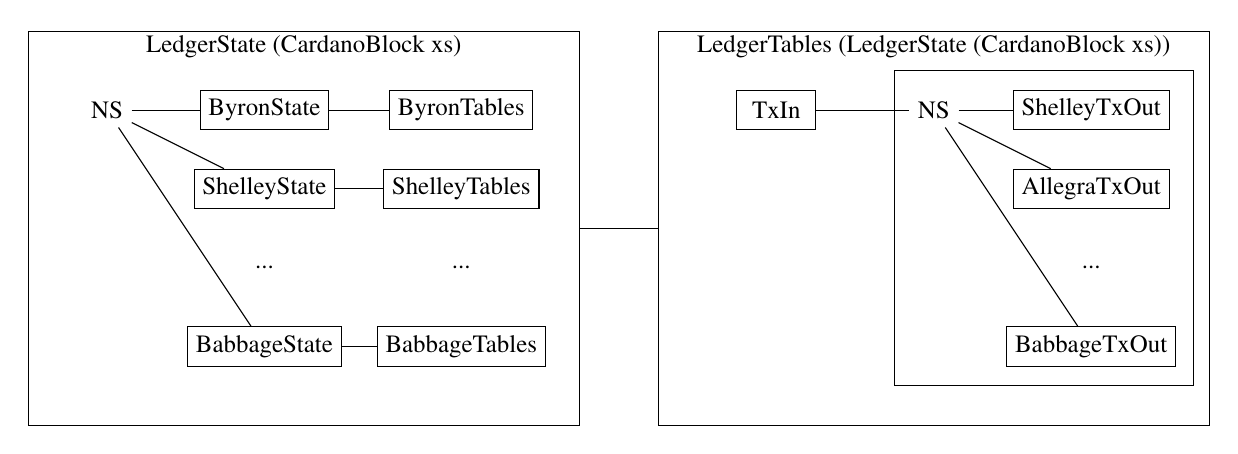
\begin{tikzpicture}
  \small
  \node at (3.5,4.8) {\small{LedgerState (CardanoBlock xs)}};
  \draw (0,0) rectangle (7,5);
  \node (oneOf2) at (1,4) [draw=none] {NS};
  \node (bb) at (3,4) [draw,minimum width=1cm,minimum height=0.5cm] {ByronState};
  \node (bt) at (5.5,4) [draw,minimum width=1cm,minimum height=0.5cm] {ByronTables};
  \node (sb) at (3,3) [draw,minimum width=1cm,minimum height=0.5cm] {ShelleyState};
  \node (st) at (5.5,3) [draw,minimum width=1cm,minimum height=0.5cm] {ShelleyTables};
  \node (db) at (3,2) [draw=none,minimum width=1cm,minimum height=0.5cm] {...};
  \node (dt) at (5.5,2) [draw=none,minimum width=1cm,minimum height=0.5cm] {...};
  \node (bab) at (3,1) [draw,minimum width=1cm,minimum height=0.5cm] {BabbageState};
  \node (bat) at (5.5,1) [draw,minimum width=1cm,minimum height=0.5cm] {BabbageTables};
  \draw (oneOf2) -> (bb);
  \draw (bb) -> (bt);
  \draw (oneOf2) -> (sb);
  \draw (sb) -> (st);
  \draw (oneOf2) -> (bab);
  \draw (bab) -> (bat);


  \draw (7,2.5) -> (8,2.5);


  \node at (11.5,4.8) {\small{LedgerTables (LedgerState (CardanoBlock xs))}};
  \draw (8,0) rectangle (15,5);
  \node (rect) at (9.5,4) [draw,minimum width=1cm,minimum height=0.5cm] {TxIn};
  \node (oneOf) at (11.5,4) [draw=none] {NS};
  \draw (rect) -> (oneOf);
  \node (sh) at (13.5,4) [draw,minimum width=1cm,minimum height=0.5cm] {ShelleyTxOut};
  \node (al) at (13.5,3) [draw,minimum width=1cm,minimum height=0.5cm] {AllegraTxOut};
  \node (my) at (13.5,2) [draw=none,minimum width=1cm,minimum height=0.5cm] {...};
  \node (ba) at (13.5,1) [draw,minimum width=1cm,minimum height=0.5cm] {BabbageTxOut};
  \draw (oneOf) -> (sh);
  \draw (oneOf) -> (al);
  \draw (oneOf) -> (ba);
  \draw (11,0.5) rectangle (14.8,4.5);
\end{tikzpicture}

So the code that is block agnostic (the whole \texttt{ouroboros-consensus}) will
carry \htt{CardanoLedgerTables} (right side on the diagram above), and when the
code unwraps the underlying ledger state inside the telescope (for example when
applying a block to a ledger state or ticking a ledger state) then it will
inject the Cardano tables into the tables of the specific era (move the values
from the right side into the left side on the diagram above).

\subsection{Era transitions}
\label{sec:eratrans}

\subsubsection{Byron to Shelley}

As Byron doesn't have tables but Shelley does, the era transition creates out of
thin air a set of differences which insert all and every value on the UTxO set
into the ledger tables. This huge set of differences will be eventually garbage
collected once the first Shelley block ends up further than $k$ blocks from the
node's tip and a flushing is performed.

\subsubsection{Shelley to Allegra}

On Byron, some addresses existed there to be reclaimed by
investors\footnote{These were called AVVM addresses. Perhaps the Ledger team can
  tell more about them}, and as some were never reclaimed, the ledger made the
decision of giving the Ada in those addresses back to the treasury. This
happened on the Allegra boundary, and therefore the ledger state has been
modified to keep track of this information so that the era transition can
consume these entries into the treasury and return a set of deletions of those
addresses on the UTxO set.

See \texttt{Cardano.Ledger.Allegra.Translation.shelleyToAllegraAVVMsToDelete}.

\bibliographystyle{acm} % We choose the "plain" reference style
\bibliography{report} % Entries are in the refs.bib file

\end{document}
